%DIF LATEXDIFF DIFFERENCE FILE


%%%%%%%%%%%%%%%%%%%%%%% file typeinst.tex %%%%%%%%%%%%%%%%%%%%%%%%%
%
% This is the LaTeX source for the instructions to authors using
% the LaTeX document class 'llncs.cls' for contributions to
% the Lecture Notes in Computer Sciences series.
% http://www.springer.com/lncs       Springer Heidelberg 2006/05/04
%
% It may be used as a template for your own input - copy it
% to a new file with a new name and use it as the basis
% for your article.
%
% NB: the document class 'llncs' has its own and detailed documentation, see
% ftp://ftp.springer.de/data/pubftp/pub/tex/latex/llncs/latex2e/llncsdoc.pdf
%
%%%%%%%%%%%%%%%%%%%%%%%%%%%%%%%%%%%%%%%%%%%%%%%%%%%%%%%%%%%%%%%%%%%


\documentclass[runningheads,a4paper]{llncs}

\usepackage{amssymb}
\setcounter{tocdepth}{3}
\usepackage{graphicx}

\usepackage{url}
\urldef{\mailsa}\path|{aahma078,msain2,elsaddik}@uottawa.ca|
\newcommand{\keywords}[1]{\par\addvspace\baselineskip
\noindent\keywordname\enspace\ignorespaces#1}
%DIF PREAMBLE EXTENSION ADDED BY LATEXDIFF
%DIF UNDERLINE PREAMBLE %DIF PREAMBLE
\RequirePackage[normalem]{ulem} %DIF PREAMBLE
\RequirePackage{color}\definecolor{RED}{rgb}{1,0,0}\definecolor{BLUE}{rgb}{0,0,1} %DIF PREAMBLE
\providecommand{\DIFadd}[1]{{\protect\color{blue}\uwave{#1}}} %DIF PREAMBLE
\providecommand{\DIFdel}[1]{{\protect\color{red}\sout{#1}}}                      %DIF PREAMBLE
%DIF SAFE PREAMBLE %DIF PREAMBLE
\providecommand{\DIFaddbegin}{} %DIF PREAMBLE
\providecommand{\DIFaddend}{} %DIF PREAMBLE
\providecommand{\DIFdelbegin}{} %DIF PREAMBLE
\providecommand{\DIFdelend}{} %DIF PREAMBLE
%DIF FLOATSAFE PREAMBLE %DIF PREAMBLE
\providecommand{\DIFaddFL}[1]{\DIFadd{#1}} %DIF PREAMBLE
\providecommand{\DIFdelFL}[1]{\DIFdel{#1}} %DIF PREAMBLE
\providecommand{\DIFaddbeginFL}{} %DIF PREAMBLE
\providecommand{\DIFaddendFL}{} %DIF PREAMBLE
\providecommand{\DIFdelbeginFL}{} %DIF PREAMBLE
\providecommand{\DIFdelendFL}{} %DIF PREAMBLE
\newcommand{\DIFscaledelfig}{0.5}
%DIF HIGHLIGHTGRAPHICS PREAMBLE %DIF PREAMBLE
\RequirePackage{settobox} %DIF PREAMBLE
\RequirePackage{letltxmacro} %DIF PREAMBLE
\newsavebox{\DIFdelgraphicsbox} %DIF PREAMBLE
\newlength{\DIFdelgraphicswidth} %DIF PREAMBLE
\newlength{\DIFdelgraphicsheight} %DIF PREAMBLE
% store original definition of \includegraphics %DIF PREAMBLE
\LetLtxMacro{\DIFOincludegraphics}{\includegraphics} %DIF PREAMBLE
\newcommand{\DIFaddincludegraphics}[2][]{{\color{blue}\fbox{\DIFOincludegraphics[#1]{#2}}}} %DIF PREAMBLE
\newcommand{\DIFdelincludegraphics}[2][]{% %DIF PREAMBLE
\sbox{\DIFdelgraphicsbox}{\DIFOincludegraphics[#1]{#2}}% %DIF PREAMBLE
\settoboxwidth{\DIFdelgraphicswidth}{\DIFdelgraphicsbox} %DIF PREAMBLE
\settoboxtotalheight{\DIFdelgraphicsheight}{\DIFdelgraphicsbox} %DIF PREAMBLE
\scalebox{\DIFscaledelfig}{% %DIF PREAMBLE
\parbox[b]{\DIFdelgraphicswidth}{\usebox{\DIFdelgraphicsbox}\\[-\baselineskip] \rule{\DIFdelgraphicswidth}{0em}}\llap{\resizebox{\DIFdelgraphicswidth}{\DIFdelgraphicsheight}{% %DIF PREAMBLE
\setlength{\unitlength}{\DIFdelgraphicswidth}% %DIF PREAMBLE
\begin{picture}(1,1)% %DIF PREAMBLE
\thicklines\linethickness{2pt} %DIF PREAMBLE
{\color[rgb]{1,0,0}\put(0,0){\framebox(1,1){}}}% %DIF PREAMBLE
{\color[rgb]{1,0,0}\put(0,0){\line( 1,1){1}}}% %DIF PREAMBLE
{\color[rgb]{1,0,0}\put(0,1){\line(1,-1){1}}}% %DIF PREAMBLE
\end{picture}% %DIF PREAMBLE
}\hspace*{3pt}}} %DIF PREAMBLE
} %DIF PREAMBLE
\LetLtxMacro{\DIFOaddbegin}{\DIFaddbegin} %DIF PREAMBLE
\LetLtxMacro{\DIFOaddend}{\DIFaddend} %DIF PREAMBLE
\LetLtxMacro{\DIFOdelbegin}{\DIFdelbegin} %DIF PREAMBLE
\LetLtxMacro{\DIFOdelend}{\DIFdelend} %DIF PREAMBLE
\DeclareRobustCommand{\DIFaddbegin}{\DIFOaddbegin \let\includegraphics\DIFaddincludegraphics} %DIF PREAMBLE
\DeclareRobustCommand{\DIFaddend}{\DIFOaddend \let\includegraphics\DIFOincludegraphics} %DIF PREAMBLE
\DeclareRobustCommand{\DIFdelbegin}{\DIFOdelbegin \let\includegraphics\DIFdelincludegraphics} %DIF PREAMBLE
\DeclareRobustCommand{\DIFdelend}{\DIFOaddend \let\includegraphics\DIFOincludegraphics} %DIF PREAMBLE
\LetLtxMacro{\DIFOaddbeginFL}{\DIFaddbeginFL} %DIF PREAMBLE
\LetLtxMacro{\DIFOaddendFL}{\DIFaddendFL} %DIF PREAMBLE
\LetLtxMacro{\DIFOdelbeginFL}{\DIFdelbeginFL} %DIF PREAMBLE
\LetLtxMacro{\DIFOdelendFL}{\DIFdelendFL} %DIF PREAMBLE
\DeclareRobustCommand{\DIFaddbeginFL}{\DIFOaddbeginFL \let\includegraphics\DIFaddincludegraphics} %DIF PREAMBLE
\DeclareRobustCommand{\DIFaddendFL}{\DIFOaddendFL \let\includegraphics\DIFOincludegraphics} %DIF PREAMBLE
\DeclareRobustCommand{\DIFdelbeginFL}{\DIFOdelbeginFL \let\includegraphics\DIFdelincludegraphics} %DIF PREAMBLE
\DeclareRobustCommand{\DIFdelendFL}{\DIFOaddendFL \let\includegraphics\DIFOincludegraphics} %DIF PREAMBLE
%DIF END PREAMBLE EXTENSION ADDED BY LATEXDIFF

\begin{document}

\mainmatter  % start of an individual contribution

% first the title is needed
\title{A Proxemic Multimedia Interaction over the\\Internet of Things}

% a short form should be given in case it is too long for the running head
\titlerunning{Lecture Notes in Computer Science: Authors' Instructions}

% the name(s) of the author(s) follow(s) next
%
% NB: Chinese authors should write their first names(s) in front of
% their surnames. This ensures that the names appear correctly in
% the running heads and the author index.
%
\author{\DIFdelbegin \DIFdel{Ali Danesh}\DIFdelend \DIFaddbegin \DIFadd{Shiva suthapalli}\DIFaddend %
\and \DIFdelbegin \DIFdel{Mukesh Saini}\DIFdelend \DIFaddbegin \DIFadd{Gurukaranpreet singh}\DIFaddend \and  \DIFdelbegin \DIFdel{Abdulmotaleb El Saddik}\DIFdelend \DIFaddbegin \DIFadd{Himanshu parihar}\DIFaddend }%
% (feature abused for this document to repeat the title also on left hand pages)

% the affiliations are given next; don't give your e-mail address
% unless you accept that it will be published
\institute{MCRLab, University of Ottawa, Ottawa ON K1N 6N5, Canada\\
\mailsa\\
\mailsb\\
\mailsc\\
\url{http://www.mcrlab.uottawa.ca/}}

%
% NB: a more complex sample for affiliations and the mapping to the
% corresponding authors can be found in the file "llncs.dem"
% (search for the string "\mainmatter" where a contribution starts).
% "llncs.dem" accompanies the document class "llncs.cls".
%

\toctitle{Lecture Notes in Computer Science}
\tocauthor{Authors' Instructions}
\maketitle


\begin{abstract}
With the rapid growth of online devices, a new concept of
Internet of Things (IoT) is emerging in which everyday devices will be connected to the Internet. As the number of devices in IoT is increasing, so is the complexity of the interactions between user and devices. There is a need to design intelligent user interfaces that could assist users in interactions. The present study proposes a proximity-based user interface for multimedia devices over IoT. The proposed method employs a cloud-based decision engine to support user to choose and interact with the most appropriate device, reliving the user from the burden of enumerating available devices manually. The decision engine observes the multimedia content and device properties, learns user preferences adaptively, and automatically recommends the most appropriate device to interact. The system evaluation shows that the users agree with the proposed interaction 70\% of the times.
\DIFaddbegin 

\DIFadd{EXAMPLE SENTENCE I ADDED
}\DIFaddend \keywords{Proxemic interaction; multimedia interaction ; user interface; elicitation study}
\end{abstract}


\section{Introduction}

The Internet has been expanding very rapidly with time. Now, more than 2.7
billion people (almost 39% of world’s population) have access to it and use it in
their daily life [1]. The number of devices that are connected to the Internet has
been growing dramatically. Therefore, a new concept of Internet of Things (IoT)
is emerging [2]. More than 11.2 billion devices were connected to the Internet in
2013 and it is predicted that there will be around 50 billion devices online by 2020
[3]. These uniquely identifiable objects and devices move and interact with each
other to accomplish various tasks. In other words, IoT is like a big and dynamic
society of objects and people. But we are far from the ubiquitous computing
vision of Weiser [4] due to two main reasons: the lack of an appropriate taskcentered User Interface (UI) design approach and the lack of reliable support
for distributable user interfaces in ubiquitous environments [5]. Thus, there is a
need for a new generation of specifically designed user interfaces for IoT.



More than 7 billion people constantly use verbal and nonverbal communication techniques to interact with their society all across the world. Verbal communication is considered as the main channel since it is used explicitly. However,nonverbal communication such as Proxemics, Haptics, Body Language, etc. plays
an important role in the human society because it uses implicit interactions. In
the same way, nonverbal communication can also enhance the interactions within
the IoT, which is ike human’s society except the size of IoT is few times bigger
than human society. Thus, nonverbal techniques should be used in order to build
proper user interfaces for ubiquitous environments, particularly the IoT.



The present study proposes a distributed user interface that provides a suitable environment for multimedia interactions over the IoT. It consists of a cloudbased decision engine that manages the proxemic interactions. This engine is
called Proxemic Interaction Unit (PIU). PIU uses multimedia devices within
the IoT as elements of a universal UI in order to assist users to make use of
their surrounding devices. We collected some of the effectual multimedia interaction variables such as device properties, multimedia content attributes, user’s
preferences, etc. to propose a scoring mechanism for the PIU. A group of these
variables are obtained by conducting a user survey and elicitation study while
the rest are extracted from the literature. To further personalize user preferences,
we update the variables after every interaction. The evaluation shows that 70%
of the times the user interface chooses the same device a user would. We reckon
that the user preference learning mechanism will further increase the accuracy
of the user interface.



The rest of this paper firstly presents a review of related works in Section
2. Next, Section 3 describes the architecture and details of proposed UI. The
results of an evaluation user study are given in Section 4, which is followed by
brief discussion in Section 5. This study ends with the conclusion and future
work in Section 6.
\DIFaddbegin \DIFadd{Don't cry because it's over, smile because it happened.
}\DIFaddend 

\section{Related Work}
Researchers have been trying to develop new UIs over the IoT for the last few
years. However, the idea of using proxemic interactions has been around for
a while. Hall highlighted the influence of proxemic behavior on interpersonal
communication in 1966 [6]. He divided proxemic interactions into two levels:
micro-level, which studies the way people interact with each other in daily life
and macro-level, which reviews the space organization of houses, buildings and
ultimately towns. More recently, Greenberg et al. proposed a practical version
of proxemic interaction that considers people, digital devices, and non-digital
objects [7]. They defined five dimensions for proxemic interaction: distance, orientation, movement, identity, and location. Every measured change in any dimension can trigger an interaction. Marquardt et al. used this terminology to
develop a proximity toolkit in order to aid fast prototyping of proxemic interactions [8]. Despite the fact that researchers have been trying to define a more
precise structure and terminology for proxemic interactions recently, proxemics
have been involved in applications for a long time.



Researchers study the interactions between smart objects in the IoT (e.g. [9]). However, the research community has paid more attention to the human-device.interactions (e.g. [10, 11]). Ju et al. proposed the Range as a public interactive
whiteboard, which supports co-located, ad-hoc meetings [12]. It uses the proximity sensing to proactively manage the transitions between display and authors
(e.g. to clear the space for writing). Wang et al. introduced Proxemic Peddler,
which is a public display [13]. This public display can capture and preserve the
attention of pedestrians. Both of the aforementioned studies are examples of
human-device proxemic interactions in micro-level where the proximity space
is very small (e.g. one room). Researchers also have developed some proximity
aware applications at macro-level (e.g. multiple rooms). The active badge, which
was introduced by Want et al., is one of them [14]. They embedded an infrared
beacon into their badge in order to connect it to a sensory network. Using this
architecture, they could track employees in the office and redirect their phone
calls to their current stations. Active badge was successfully implemented and
used in large scale.



Moreover, there are some studies that focus on possible human-device proxemic interactions in households. The EasyLiving is one of the earliest projects
in this group [15]. It emphasizes on an architecture, which can connect different
devices together in order to enhance the user experience. Ramani et al. proposed
a new location tracking system for media appliances in the wireless home networks, which can be used to build a proxemic media redirection system [16].
Recently, Sørensen et al. introduced and evaluated the AirPlayer, which is a
multi-room music system that uses the proxemic interaction [17].



In conclusion, there is no custom designed proxemic interface for multimedia
interactions. The proposed UI is designed and optimized for proxemic multimedia interaction, which makes it a task-specific UI. Furthermore, we believe that
a completely distributed solution (e.g. [17]) cannot meet the growing requirements of the IoT users. Therefore, the proposed method employs a cloud-based
decision engine (PIU), which considers additional information such as multimedia content properties, user’s preferences, devise capabilities etc. in order to
improve multimedia interactions. Moreover, the current trend is that a cloudbase database keeps the shared resources including multimedia data. Hence, our
design of a cloud-based decision engine is in accordance with the current technological trends.
\DIFdelbegin %DIFDELCMD < 

%DIFDELCMD < %%%
\DIFdelend \DIFaddbegin \DIFadd{I'm selfish, impatient and a little insecure. I make mistakes, I am out of control and at times hard to handle. But if you can't handle me at my worst, then you sure as hell don't deserve me at my best.
}\DIFaddend \section{Proposed System}
The main purpose of the proposed UI is to provide an environment within the
IoT that supports the proxemic interactions for multimedia devices. The proposed system has three main components: proxemic interaction unit (PIU), media redirection unit, and tracking engine. PIU is the central part of the system.
Figure 1 presents the abstract algorithm of PIU. As we can see in the figure, the
algorithm begins by receiving the location information of the devices. PIU uses
the tracking engine to find the locations and update it on the location database.
Next, PIU  checks for possible proxemic interaction. Then PIU calculates a score
between 0 and 1 for each device based on content properties, user preferences,and device capabilities. Consequently, the algorithm finds the device with maximum score. If it is not the same device as the one in use, it notifies the user and
recommends a media redirection. If user accepts the recommendation, PIU asks
the media redirection unit to handle this process. After each interaction, PIU
updates the scoring coefficients to learn user’s preferences adaptively.
\DIFaddbegin \DIFadd{Be yourself; everyone else is already taken.
}\DIFaddend 

\begin{figure}[h]
\centering
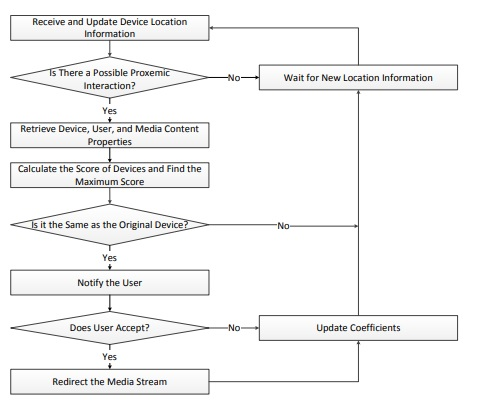
\includegraphics[width=1\textwidth]{fig1.jpg}
\caption{The abstract algorithm of proxemic interaction unit.}
\end{figure}
The device scoring and recommendation step in the aforementioned algo-
rithm is the most important step since it can assist users to engage with a larger
number of devices in the IoT. To recommend the most appropriate device in the
given scenario, we should find and imply different variables in the scoring mech-
anism. Therefore, we start by introducing these variables and then present the
scoring mechanism. There are three groups involved in the proposed solution:
devices, users, and multimedia content. Below we study these groups in order to
find effective variables for the scoring mechanism.
\DIFaddbegin \DIFadd{Two things are infinite: the universe and human stupidity; and I'm not sure about the universe.
}\DIFaddend 



\subsection{Devices}

Devices are the first and most important objects in our system. Since the proposed system provides an environment for proxemic interactions, we begin by
explaining device’s proximity behavior. Hall defined four perimeters around each
person: intimate space, personal space, social space, and public space (Table 1)
[6]. We are using same categorization for devices according to their effective quality in each space: intimate devices, personal devices, social devices, and public
devices. For example, smartphones have small screens, so they are usually used
by individuals separately. Moreover, they have the best visual quality when they
are close to the user (e.g. 20 cm which is in the intimate space). Users can still
see the smartphone screen when they are farther away, but their effective quality decreases. Similarly, users enjoy big screen TVs most when they are at an
acceptable distance, i.e., 3.5 m to 6 m. Hence, they are placed in the category
of public devices. Let T(x) be a function that returns an integer between 0 to 3
depending on the type of device x. Table 1 provides examples of all 4 groups of
device spaces and function T() value for each device type. We will use function
T() later while calculating scored for each device.
\DIFaddbegin \DIFadd{So many books, so little time.
}\DIFaddend 

\begin{tabular}{ |p{2.5cm}||p{3.7cm}|p{3.7cm}|p{0.7cm}|  }
 \hline
 \hline
 Space Name& Space Area &Device Examples &T ()\\
 \hline
 Intimate Space   & distance \leq 0.45 &smartphones&   0\\
 Personal Space&   0.45 m\leq distance\leq 1.2 m & tablets, laptops   &1\\
 Social Space &1.2 m \leq distance \leq3.6 m & PCs, digital displays&  2\\
 Public Space    &3.6 m \leq distance \leq 7.6 m & TVs, home stereos&  3\\

 \hline
\end{tabular}




\subsection{User Survey}

It is important to characterize user priorities in order to design effective user
interface. We conducted a user survey to study user’s attitudes and preferences.
Participants had to answer 17 questions regarding the frequency of using multimedia contents, their device preferences, and satisfaction levels. We prepared
questions such that they do not require any specific domain knowledge. Due to
lack of space, we could not present the designed questionnaire here. The website
we used for the study and the questionnaire details can be found at 1
. Totally,
149 people of an average age of 28.62 years participated in our study with the
following gender distribution: 53.7\% male and 46.3\% female. They were engineers, employees, physicians, university students and professors, etc. with different background levels in IT; 53\% of them were involved in a profession that
requires a high level of IT knowledge while the other 47% were not involved in
those kinds of jobs.



Results of this user survey revealed some interesting points. First, we could
not find any correlation between the gender and device preferences. However,
when we grouped our participants into young (≤ 30 years) and old (⪈ 30 years)
users, we found that old participants are more interested in using TVs and PCs
than tablets and smartphones. In addition to that, profession had an effect on
the device preferences. Participants who were involved in jobs that need a high
level of IT knowledge were keener to use PCs and TVs. We also found that
frequent users (who spend up to 1 hour per day) prefer TVs and PCs more than
non-frequent users non-frequent users (who spend more than 1 hour per day).



To summarize, based on the results of this user survey, we were convinced to
include three characteristics of the engaged user, u, in our scoring mechanism:
participant’s age (U
a
), profession type (U
p
), and multimedia usage habits (U
h
).
We used the user ratings to initialize preference coefficients corresponding to
these characteristics, which are updated over time according to user interactions.
\DIFaddbegin \DIFadd{Be who you are and say what you feel, because those who mind don't matter, and those who matter don't mind.
}\DIFaddend 


\subsection{MUltimedia Content}

Multimedia content properties can influence the user’s decision regarding the
playback device. For example, a video content cannot be streamed to a home
stereo, which only supports audio inputs. So, the type of the content should be
considered. In addition, there is a user study that shows the length of multimedia
content can affect the user’s choice for playback device [18]. It categorizes videos
based on their length: very short videos (up to 2 minutes, e.g. social network
clips), short videos (up to 7 minutes, e.g. music videos), medium videos (up to
22 minutes, e.g. soap operas and animations), long videos (up to 45 minutes,
e.g. TV series), and very long videos (longer than 45 minutes). Results of this
study indicates that the length of the first half of videos that are played on the
smartphones over the WiFi connection is around 50 seconds while it is almost
100 seconds for tablets. This is due to several factors such as screen dimensions
and resolutions, battery capacity, etc. Hence, we decided to use three properties
of the given multimedia content, c, in our scoring mechanism: audio of content
(C
a
), video of content (C
v
), and duration of the content (C
d
). We have grouped
long and very long videos together, as a result, C
d
can take four values depending
on the length: 0 - very short, 1 - short, 2 - medium, and 4 - long.
\DIFaddbegin \DIFadd{A room without books is like a body without a soul.
}\DIFaddend 


\subsection{Scoring Mechanism}
When the PIU finds out that there is a possible proxemic interaction, it starts
the scoring mechanism. Let D = {D i |1 ≤ i ≤ n} be the set of available devices.
For the given content c and a user u, the the score of i th device, s i , is calculated
as follows:
s i = f ic × m ic × h iu × a iu × p iu × d iu
(1)
where f ic is a flag that indicates capability of device D i to play content c, m ic
is device appropriateness coefficient for the given content, h iu , a iu , and p iu are
user’s habit, age, and profession factors for the device D i . The last element is
\DIFaddbegin \DIFadd{You've gotta dance like there's nobody watching,
Love like you'll never be hurt,
Sing like there's nobody listening,
And live like it's heaven on earth
}\DIFaddend 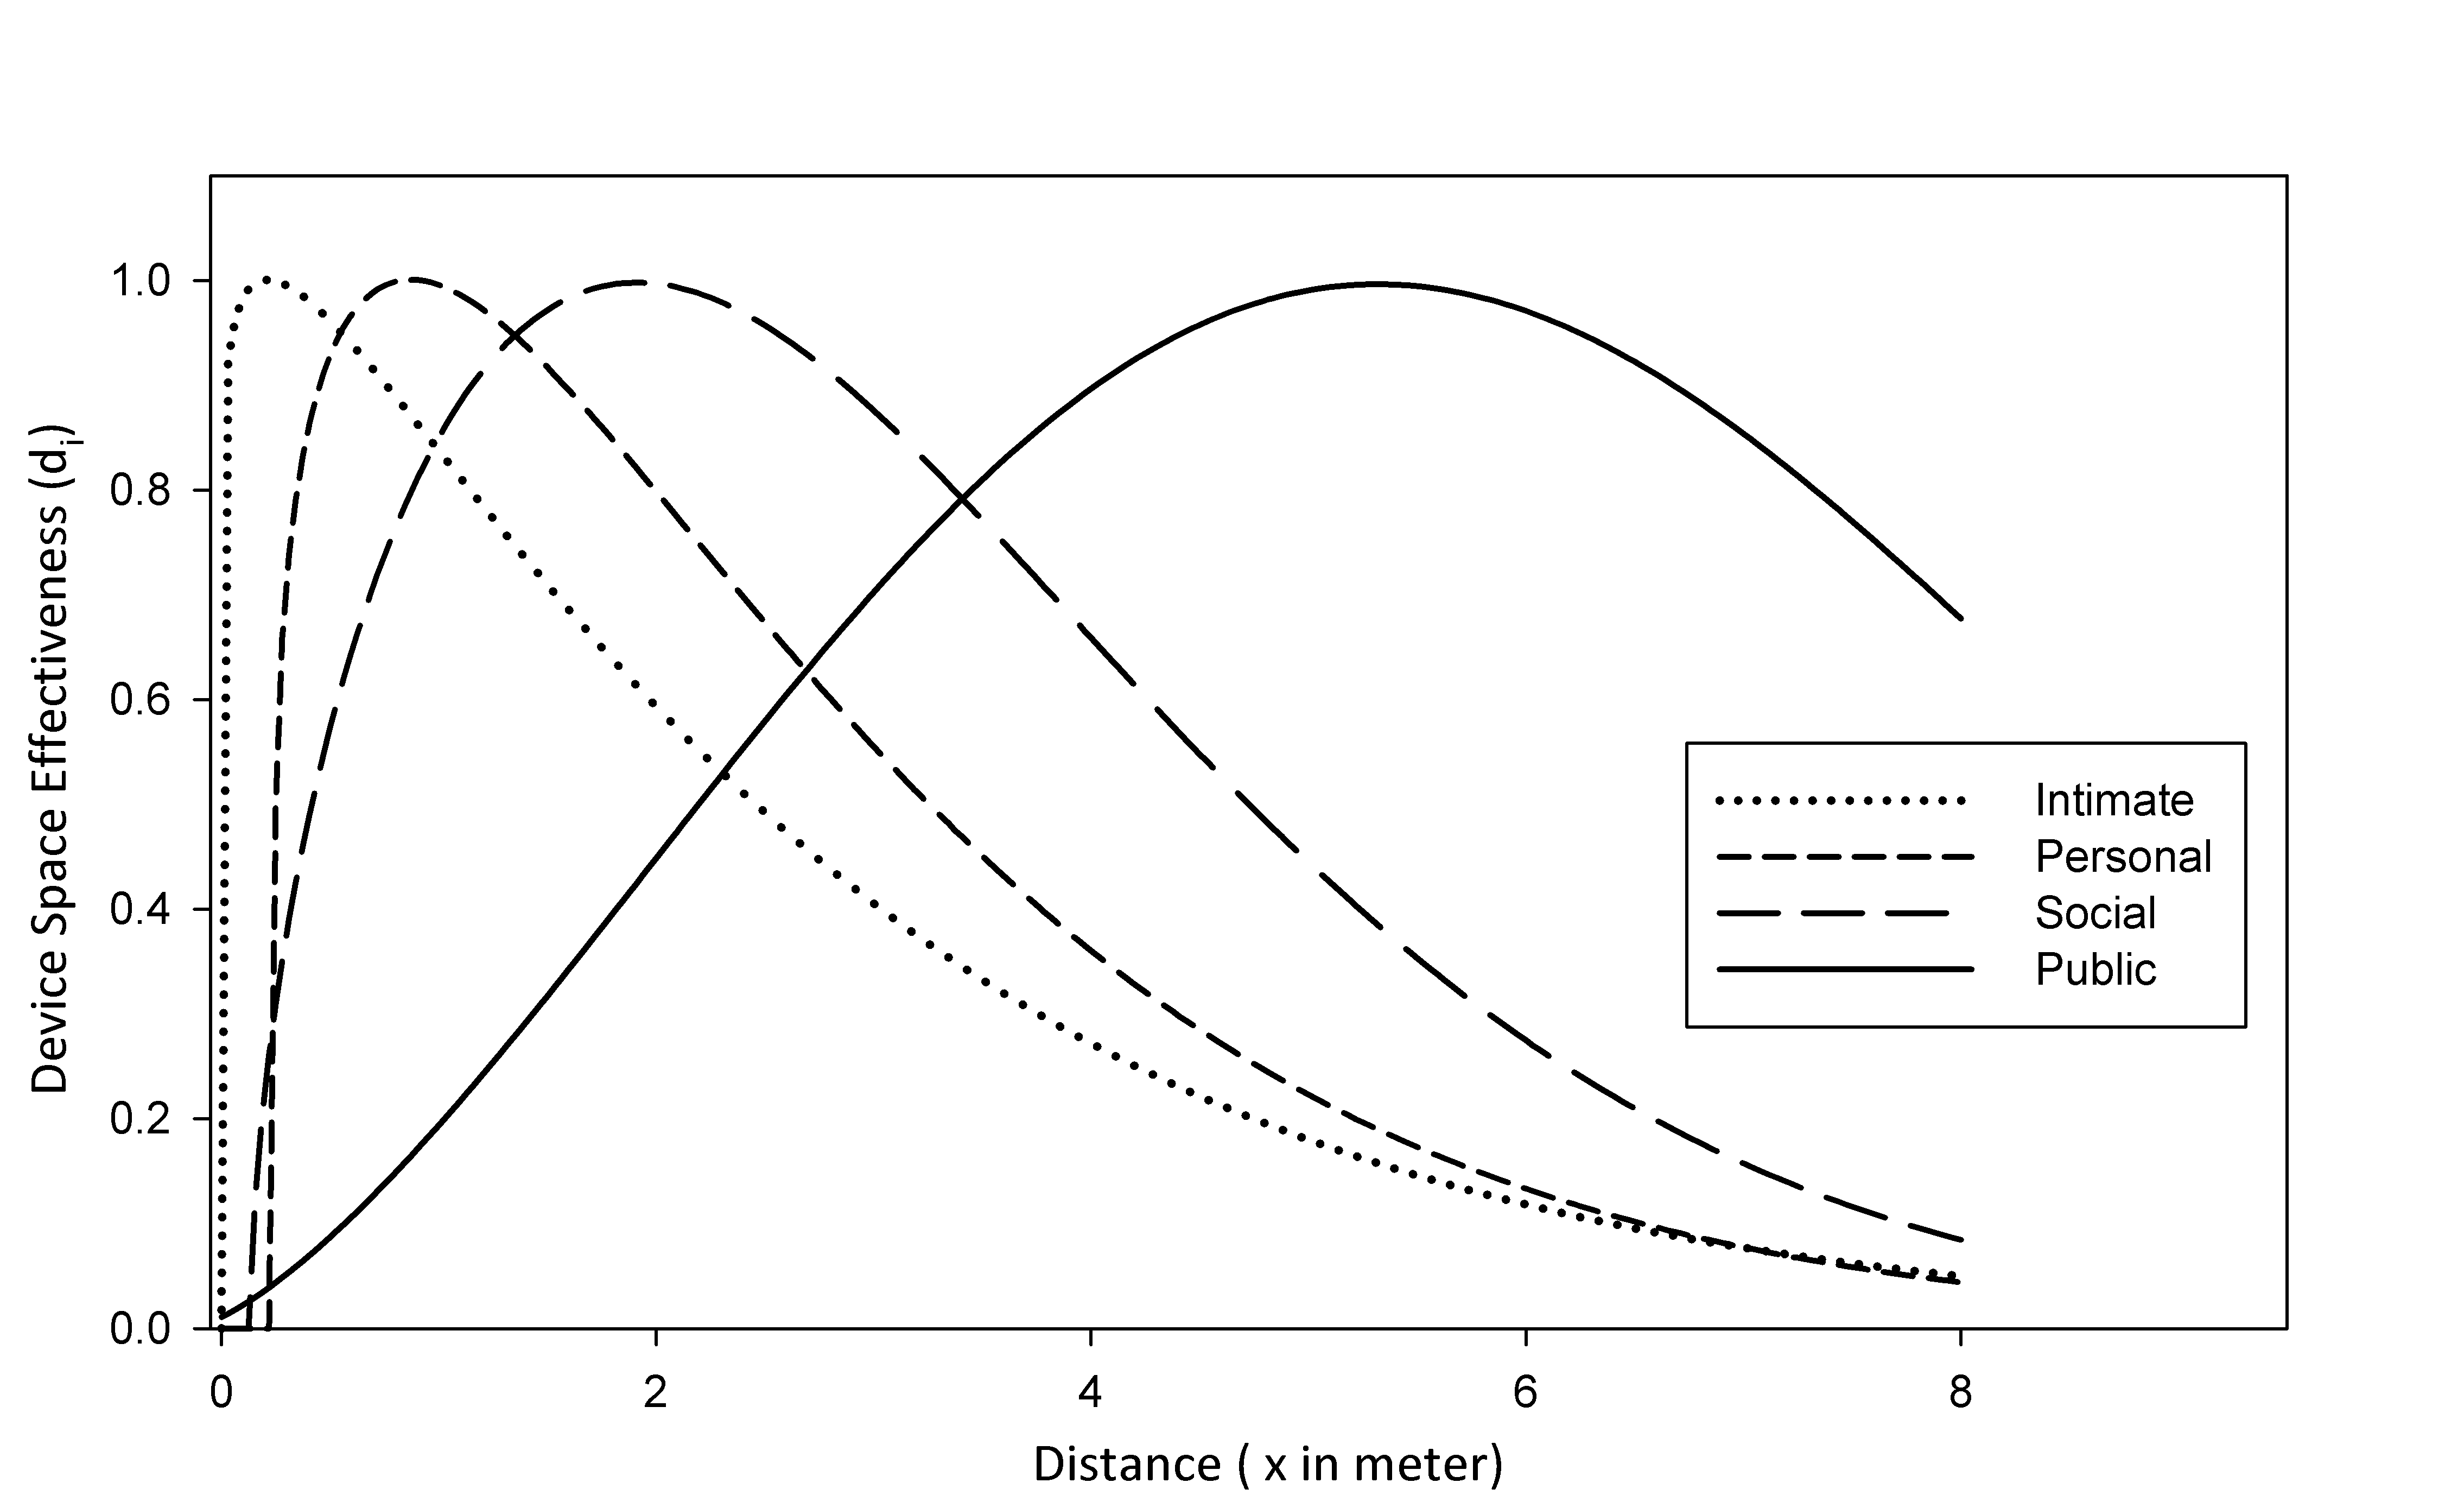
\includegraphics[scale=0.07]{fig2.png}
\subsection{Adaptation Mechanism}
The proposed solution considers different variables to calculate the score for
each device (Equation 1) in order to find the best possible device for media
redirection. Although we used the results of different surveys in order to define
the values of the coefficients in the scoring mechanism, each person may have
different preferences. Therefore, we designed an adaptation mechanism in the
proposed solution, which updates the coefficient values based on the responses
of individuals after each interaction. The PIU selects the corresponding values
for coefficients and calculates the scores. For example, imagine PIU uses user’s
age coefficient a iu to calculate the score for device D i , and D i is recommended
to the user since it has the highest score. So, when the user responds to the
recommendation, the value of a iu is updated using the following equation:


where a iu,new is the new coefficient’s value, a iu,old is the old coefficient, n r is
number of rejected recommendations for this type of device space, and n t is the
total number of recommendations for this type of device space.
\DIFaddbegin \DIFadd{You know you're in love when you can't fall asleep because reality is finally better than your dreams.
}\DIFaddend 

\section{Evaluation}
To evaluate the proposed system, we defined 4 scenarios and conducted a user
survey. In these scenarios, participants were given access to all types of devices
in their effective distance. The content’s length was the only variable in our
scenarios. In the first scenario, it was 2 min while it was 7 min, 22 min, and 90
min in the second, third and fourth scenarios respectively. As an example, the
user had to select his / her preferred device for watching a 7 min video while he
/ she has access to a smartphone in 0.25 m, tablet in 0.75 m, personal computer
in 2.5 m, and TV in 5 m. Totally, 10 people participated in our study with age
ranging from 20 to 40. The users had different professions and media playback
habits. We compared the user responses to the device recommendations made
by the proposed user interface to measure the usability.
We also compare the proposed approach with two other methods. The first
one only uses the distance to suggest a new device. So, the method always sug-
gests the device that has user in its most effective area, with the same learning
mechanism as ours. The second method is AirPlayer [17]. AirPlayer only sup-
ports intimate and public devices. Furthermore, it does not have the learning
mechanism. So, it cannot adapt itself to user’s preferences. Table 2 shows the
results of this evaluation study.
\DIFaddbegin \DIFadd{You know you're in love when you can't fall asleep because reality is finally better than your dreams.
}\DIFaddend \begin{figure}[h]
\caption{The results of the evaluation study.}
\centering
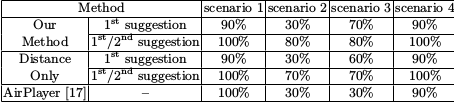
\includegraphics[width=0.7\textwidth]{fig3.png}
\end{figure}

In this study, the total accuracy of the first suggestion for our system is
equal to 70\% while it was 67.5\% for the distance only method and 62.5\% for the
AirPlayer. But, since the proposed method can learn from the users responses
and adapt itself to his / her preferences, we decided to study the accuracy of
these methods after two interactions. This is not applicable to the AirPlayer
due to its lack of learning mechanism. The total accuracy after two interactions
for our system was 90\%, however it was 85\% for the distance only method. To
summarize, we can say that the proposed method had a higher accuracy in these
scenarios. As a result, it could provide an environment that has more successful
proxemic multimedia interactions.
\subsubsection*{Acknowledgments.} The heading should be treated as a
subsubsection heading and should not be assigned a number.

\section{Discussion}

There are three points that should be discussed regarding the proposed system.
First, the proposed solution checks the identity of users by tracking their inti-
mate devices. Then, it uses their personal information to recommend a device
to them and adaptively updates itself for each user. Also, each device or user
updates the location information when it has a movement. The devices are rec-
ommended based on the distance between them. Therefore, we can conclude that
the proposed solution directly uses 3 out of 5 proxemic interaction dimensions
that were introduced earlier by Greenberg et al [7]. The remaining two dimen-
sions can be involved in this system as well. The orientation of the user and
location of devices may influence the user’s decision on playback device.

The last point is regarding the engagement mechanism. Since the number
of online devices is growing very fast, most of the times users are surrounded
by a number of devices. But, since it is not easy to migrate from one device to
the other, users may not change the device that they are using. However, the
proposed UI considers the user’s preferences and proxemic information to suggest
a new device, which can increase the number of accepted recommendations. Also,
it can assist users through the migration process by handling redirection process
in the background. Hence, the proposed UI facilitates the engagement process
for the users and provides them more options to use.
The following section shows a sample reference list with entries for
journal articles \cite{jour}, an LNCS chapter \cite{lncschap}, a book
\cite{book}, proceedings without editors \cite{proceeding1} and
\cite{proceeding2}, as well as a URL \cite{url}.
Please note that proceedings published in LNCS are not cited with their
full titles, but with their acronyms!
\section{Conclusion and Future Work}
This paper presented a new UI, which is designed for multimedia devices within
the IoT. The proposed UI provides a proxemic interaction experience to the
users. The proposed solution involves user’s preferences and media content prop-
erties in addition to the proxemic information in its scoring mechanism. Then,
it recommends a new device to the user in order to motivate him/her to engage
with the new device. The proposed algorithm adaptively trains itself towards
user’s attitude over the time based on the feedback from the user. The scoring
mechanism is validated in 4 scenarios by a user study and it has the acceptable
average accuracy of 70\%. Using the feedback from the rejection ratio, system
trains itself towards user’s attitude over the time and reaches average accuracy
of 90\%. In the future, we want to include more devices and interaction modalities
to build a generic, distributed user interface for IoT.
\DIFdelbegin %DIFDELCMD < 

%DIFDELCMD < %%%
\DIFdelend \DIFaddbegin \DIFadd{You only live once, but if you do it right, once is enough.
}\DIFaddend \begin{thebibliography}{4}

\bibitem{jour} Smith, T.F., Waterman, M.S.: Identification of Common Molecular
Subsequences. J. Mol. Biol. 147, 195--197 (1981)

\bibitem{lncschap} May, P., Ehrlich, H.C., Steinke, T.: ZIB Structure Prediction Pipeline:
Composing a Complex Biological Workflow through Web Services. In: Nagel,
W.E., Walter, W.V., Lehner, W. (eds.) Euro-Par 2006. LNCS, vol. 4128,
pp. 1148--1158. Springer, Heidelberg (2006)

\bibitem{book} Foster, I., Kesselman, C.: The Grid: Blueprint for a New Computing
Infrastructure. Morgan Kaufmann, San Francisco (1999)

\bibitem{proceeding1} Czajkowski, K., Fitzgerald, S., Foster, I., Kesselman, C.: Grid
Information Services for Distributed Resource Sharing. In: 10th IEEE
International Symposium on High Performance Distributed Computing, pp.
181--184. IEEE Press, New York (2001)

\bibitem{proceeding2} Foster, I., Kesselman, C., Nick, J., Tuecke, S.: The Physiology of the
Grid: an Open Grid Services Architecture for Distributed Systems
Integration. Technical report, Global Grid Forum (2002)

\bibitem{url} National Center for Biotechnology Information, \url{http://www.ncbi.nlm.nih.gov}

\end{thebibliography}


\section*{Appendix: Springer-Author Discount}

LNCS authors are entitled to a 33.3\% discount off all Springer
publications. Before placing an order, the author should send an email, 
giving full details of his or her Springer publication,
to \url{orders-HD-individuals@springer.com} to obtain a so-called token. This token is a
number, which must be entered when placing an order via the Internet, in
order to obtain the discount.

\section{Checklist of Items to be Sent to Volume Editors}
Here is a checklist of everything the volume editor requires from you:


\begin{itemize}
\settowidth{\leftmargin}{{\Large$\square$}}\advance\leftmargin\labelsep
\itemsep8pt\relax
\renewcommand\labelitemi{{\lower1.5pt\hbox{\Large$\square$}}}

\item The final \LaTeX{} source files
\item A final PDF file
\item A copyright form, signed by one author on behalf of all of the
authors of the paper.
\item A readme giving the name and email address of the
corresponding author.
\end{itemize}
\end{document}
